%!TEX root = ../GLM_Becerra_Lopez.tex

\section*{Apéndice: convergencia de cadenas}
\label{sec:appendix}

En esta sección, se ilustra la convergencia del proceso iterativo de MCMC de los modelos. Todos los modelos fueron corridos en JAGS versión 4.2.0\footnote{\url{http://mcmc-jags.sourceforge.net/}} llamándolo desde \texttt{R} \cite{ihaka1996r} a través del paquete \texttt{R2jags} \cite{su2015r2jags}. Cada modelo fue corrido con cuatro cadenas con puntos iniciales aleatorios. Para los modelos de unidades iguales y de unidades independientes, el tamaño de muestra era de 4000, mientras que para el modelo multinivel, se utilizó un tamaño de muestra de 8000.

Para cada modelo, se muestra primero una gráfica de cada parámetro y el valor del estadístico de convergencia de Gelman y Rubin $\hat{R}$ \cite{gelman2014bayesian} \cite{kruschke2014doing}. La idea de este estadístico es inicializar varias cadenas en distintos puntos, y después de cierto tiempo, si las cadenas convergieron, deben de tener un valor de $\hat{R}$ cercano a 1. \citeauthor{brooks1998general} recomiendan como regla de dedo un valor cercano a 1.2 \cite{brooks1998general}. Después se muestra una gráfica de este mismo estadístico, pero para las distribuciones predictivas del conjunto de entrenamiento y del conjunto de prueba. La mayoría de las cadenas tuvieron un valor menor a 1.2, y los pocos que no, estaban solamente un poco por arriba de ese valor.

También se muestran gráficas del tamaño de muestra efectivo de cada parámetro y de las distribuciones predictivas; con una línea punteada horizontal marcando el tamaño de muestra real. El tamaño de muestra efectivo tiene que ver con la autocorrelación de las cadenas, y es importante cuando se hacen inferencias, sobre todo inferencias de intervalos de probabilidad muy altos. Por ejemplo, si se desea un intervalo de probabilidad de la distribución predictiva al 99\%, entonces se requiere un tamaño de muestra efectivo grande. En general, el tamaño de muestra efectivo no fue chico, aunque hubo varios parámetros que estuvieron lejos del tamaño de muestra observado. Sin embargo, como en este trabajo no se hicieron inferencias tan precisas, no se requería un valor muy grande.


\subsection*{Modelo de unidades iguales}

\begin{figure}[H]
    \centering
    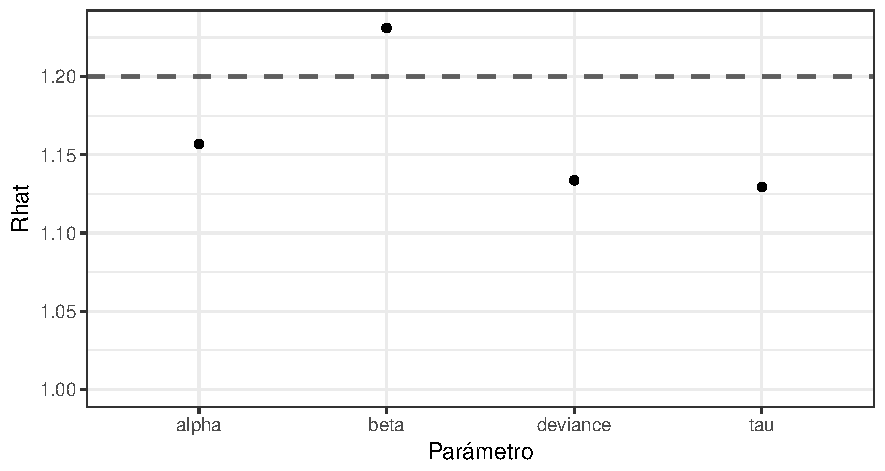
\includegraphics[width=0.9\textwidth]{images/comp_pooling_r_statistic_params.pdf}
    \caption{Estadística de convergencia $\hat{R}$ de Gelman y Rubin para cada parámetro del modelo de unidades iguales}
    \label{fig:comp_pooling_r_statistic_params}
\end{figure}

\begin{figure}[H]
    \centering
    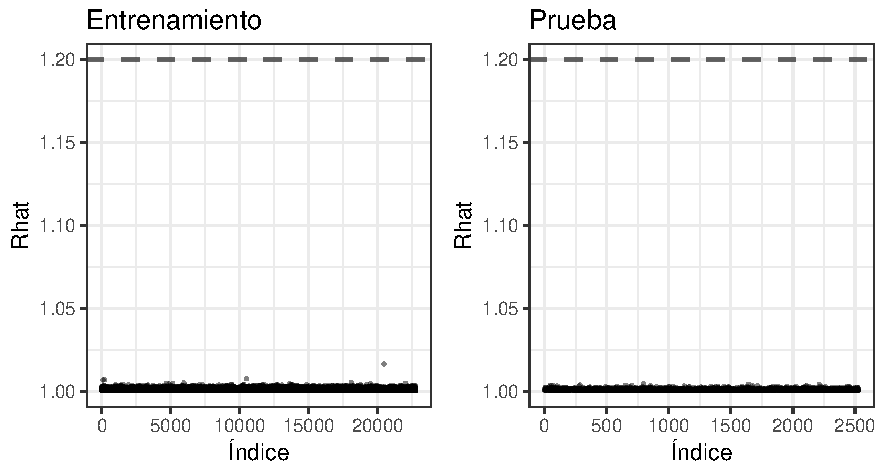
\includegraphics[width=0.9\textwidth]{images/comp_pooling_r_statistic_yf.pdf}
    \caption{Estadística de convergencia $\hat{R}$ de Gelman y Rubin para estimaciones de la variable respuesta del modelo de unidades iguales}
    \label{fig:comp_pooling_r_statistic_yf}
\end{figure}

\begin{figure}[H]
    \centering
    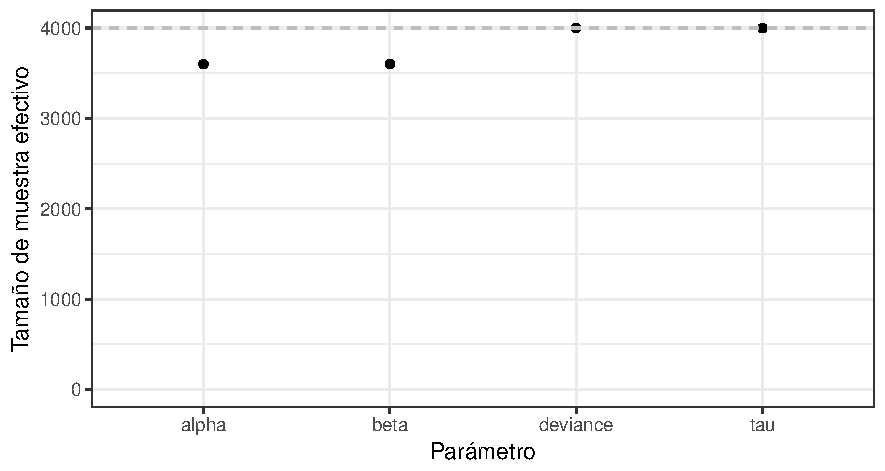
\includegraphics[width=0.9\textwidth]{images/comp_pooling_n_eff_params.pdf}
    \caption{Tamaño de muestra efectivo para cada parámetro del modelo de unidades iguales}
    \label{fig:comp_pooling_n_eff_params}
\end{figure}

\begin{figure}[H]
    \centering
    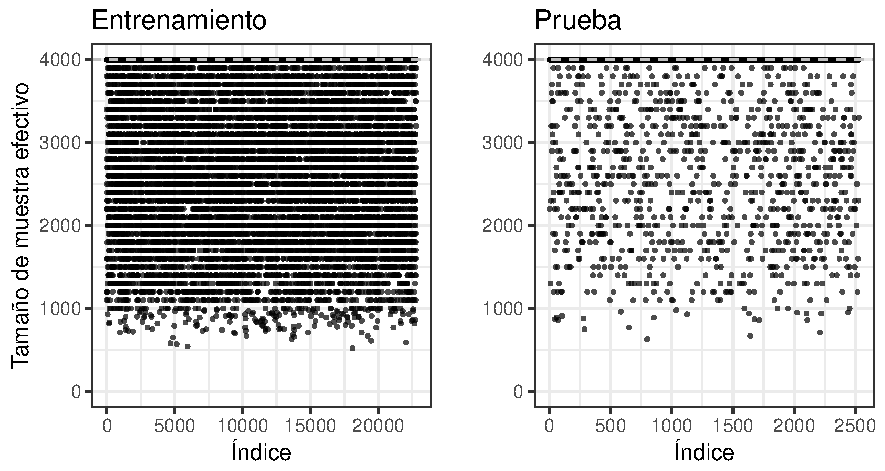
\includegraphics[width=0.9\textwidth]{images/comp_pooling_n_eff_yf.pdf}
    \caption{Tamaño de muestra efectivo para cada estimación de la variable respuesta del modelo de unidades iguales}
    \label{fig:comp_pooling_n_eff_yf}
\end{figure}



\subsection*{Modelo de unidades independientes}

\begin{figure}[H]
    \centering
    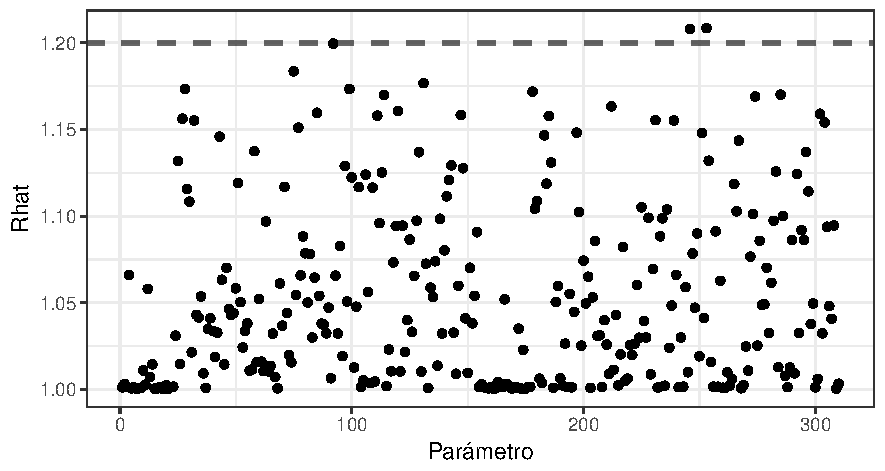
\includegraphics[width=0.9\textwidth]{images/no_pooling_r_statistic_params.pdf}
    \caption{Estadística de convergencia $\hat{R}$ de Gelman y Rubin para cada parámetro del modelo de unidades independientes}
    \label{fig:no_pooling_r_statistic_params}
\end{figure}

\begin{figure}[H]
    \centering
    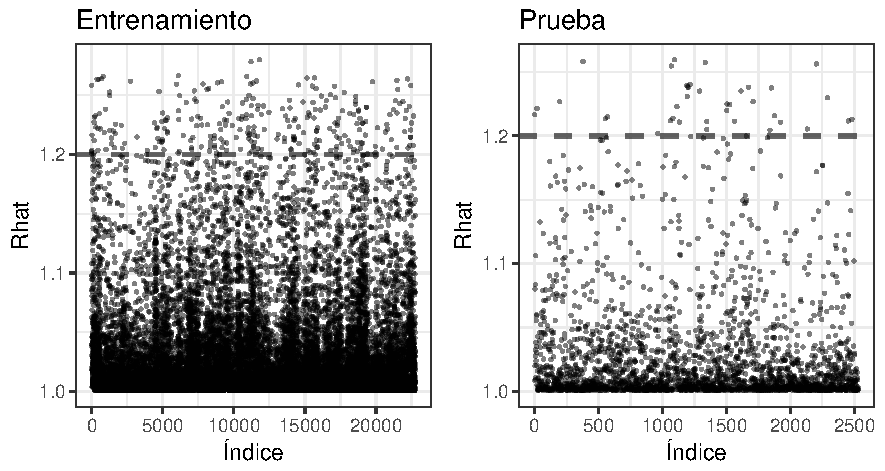
\includegraphics[width=0.9\textwidth]{images/no_pooling_r_statistic_yf.pdf}
    \caption{Estadística de convergencia $\hat{R}$ de Gelman y Rubin para estimaciones de la variable respuesta del modelo de unidades independientes}
    \label{fig:no_pooling_r_statistic_yf}
\end{figure}

\begin{figure}[H]
    \centering
    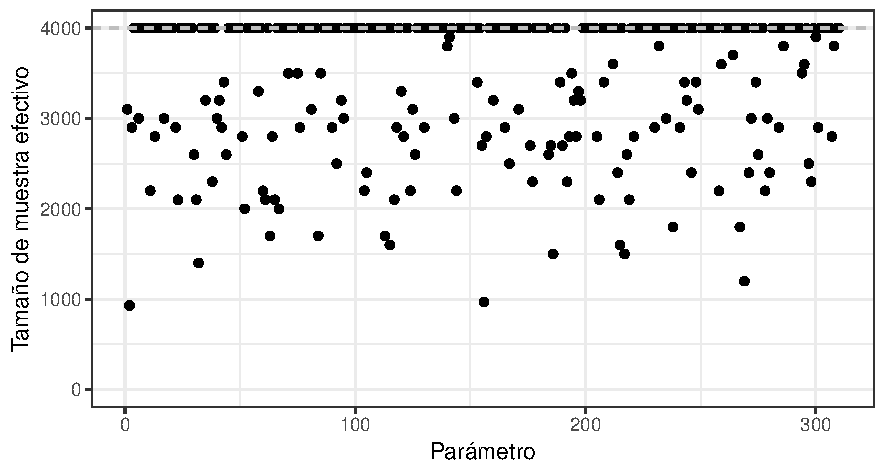
\includegraphics[width=0.9\textwidth]{images/no_pooling_n_eff_params.pdf}
    \caption{Tamaño de muestra efectivo para cada parámetro del modelo de unidades independientes}
    \label{fig:no_pooling_n_eff_params}
\end{figure}

\begin{figure}[H]
    \centering
    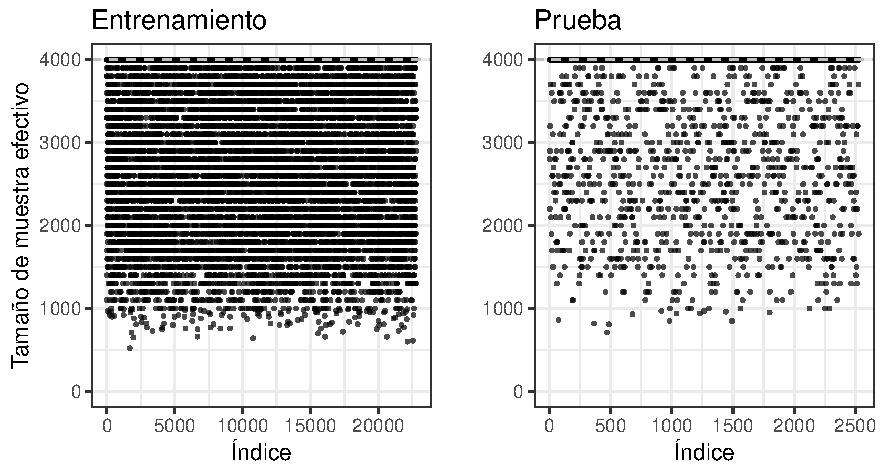
\includegraphics[width=0.9\textwidth]{images/no_pooling_n_eff_yf.pdf}
    \caption{Tamaño de muestra efectivo para cada estimación de la variable respuesta del modelo de unidades independientes}
    \label{fig:no_pooling_n_eff_yf}
\end{figure}




\subsection*{Modelo multinivel}

\begin{figure}[H]
    \centering
    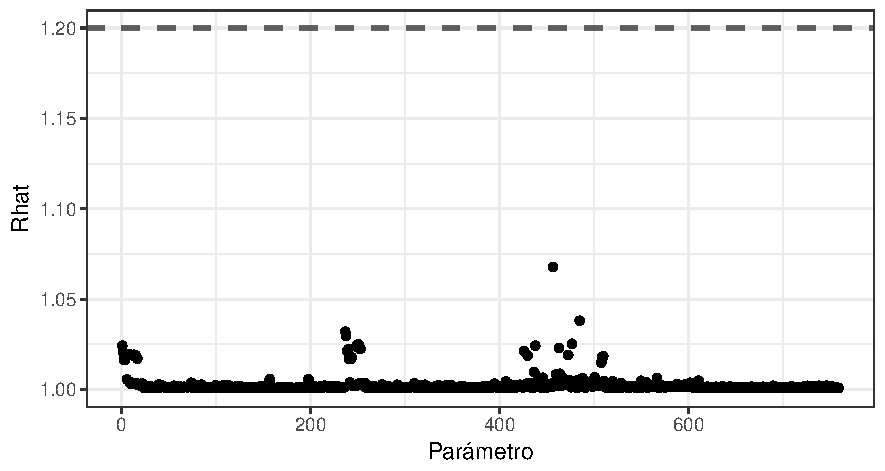
\includegraphics[width=0.9\textwidth]{images/three_levels_r_statistic_params.pdf}
    \caption{Estadística de convergencia $\hat{R}$ de Gelman y Rubin para cada parámetro del modelo multinivel}
    \label{fig:three_levels_r_statistic_params}
\end{figure}

\begin{figure}[H]
    \centering
    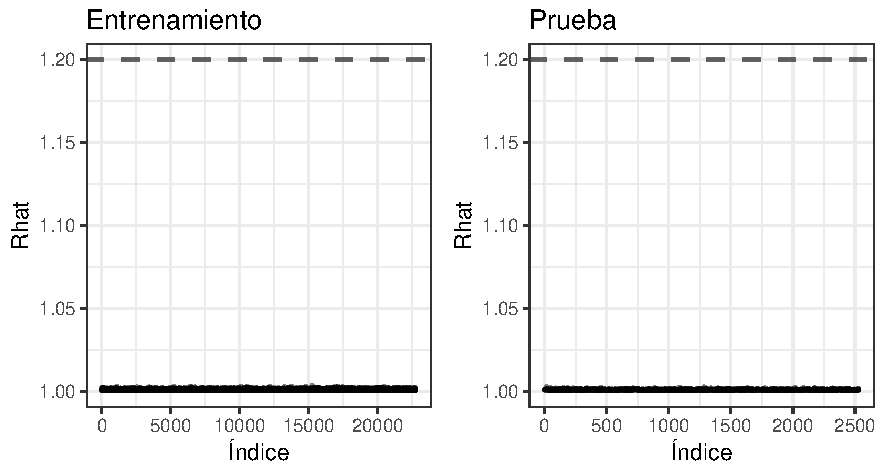
\includegraphics[width=0.9\textwidth]{images/three_levels_r_statistic_yf.pdf}
    \caption{Estadística de convergencia $\hat{R}$ de Gelman y Rubin para estimaciones de la variable respuesta del modelo multinivel}
    \label{fig:three_levels_r_statistic_yf}
\end{figure}

\begin{figure}[H]
    \centering
    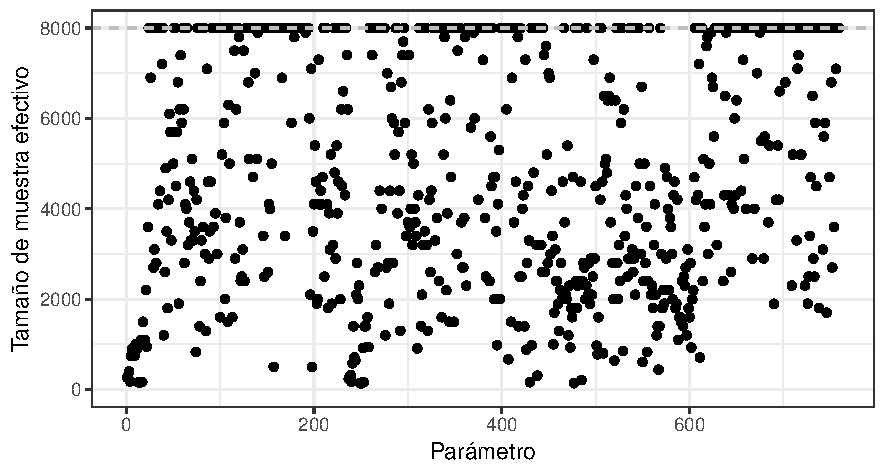
\includegraphics[width=0.9\textwidth]{images/three_levels_n_eff_params.pdf}
    \caption{Tamaño de muestra efectivo para cada parámetro del modelo multinivel}
    \label{fig:three_levels_n_eff_params}
\end{figure}

\begin{figure}[H]
    \centering
    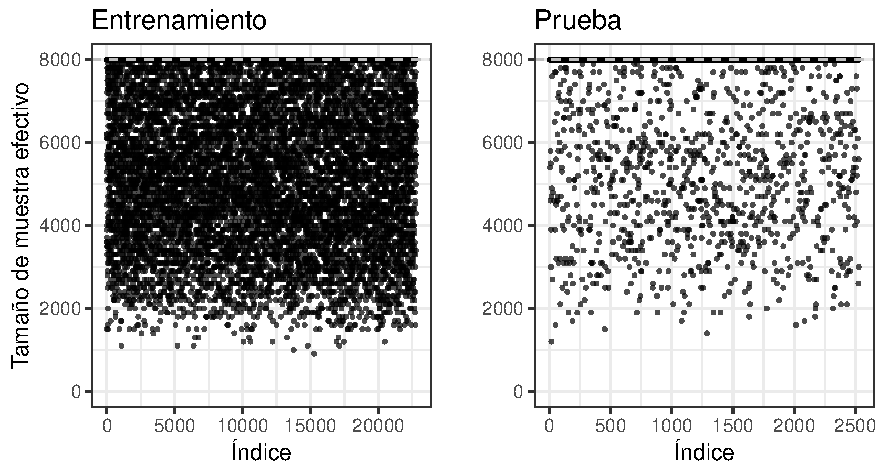
\includegraphics[width=0.9\textwidth]{images/three_levels_n_eff_yf.pdf}
    \caption{Tamaño de muestra efectivo para cada estimación de la variable respuesta del modelo multinivel}
    \label{fig:three_levels_n_eff_yf}
\end{figure}